\documentclass{easychair}

\usepackage{amsmath}
\usepackage{amssymb}
\usepackage{booktabs}
\usepackage{graphicx}
\usepackage{multirow}
\usepackage[subrefformat=parens]{subcaption}

\graphicspath{{./imgs/}}

\title{%
    Minimizing State Space Partitionings Using Decision Trees
}

\titlerunning{%
    Minimizing State Space Partitionings
}

\author{%
    Andreas Holck Høeg-Petersen\inst{1}
    \and
    Kim Guldstrand Larsen\inst{1}
    \and
    Peter Gjøl Jensen\inst{1}
    \and
    Andrzej Wasowski\inst{2}
}

\authorrunning{%
    A. H. Høeg-Petersen et.\ al.
}

\institute{%
    Aalborg University, Aalborg, Denmark \\
    \email{ahhp@cs.aau.dk, kgl@cs.aau.dk, pgj@cs.aau.dk}
    \and
    IT University of Copenhagen, Copenhagen, Denmark \\
    \email{wasowski@itu.dk}
}

\begin{document}

\maketitle

\noindent
When synthesizing safe and near-optimal control strategies for hybrid systems,
an important issue is how to deal with the continuous behavior of the system.
Generally, this can either be handled with function approximation
(eg.\ neural networks), which comes with the disadvantage of being inherently
difficult to verify, or by discretizing the continuous state space. In the
latter case, the state space is partitioned into a number of regions that are
mapped to a control action.

Such partitionings will often become overwhelmingly large as very fine-grained
partitioning is typically required to retain the necessary information for the
synthesis of a safe and optimal controller. Unfortunately, a fine-grained
partitioning will also store a lot of redundant information. For
high-dimensional state spaces, the problem grows exponentially as it falls
victim to `the curse of
dimensionality'~\cite{bellmanAdaptiveControlProcesses1959}. This can be
detrimental for both the speed of execution and for memory consumption when the
controller is expected to run on smaller, embedded devices (eg.\ to control a
pump at a water basin or a traffic light at a crossing).

We propose a novel algorithm for minimizing such mapped partitionings by
using decision trees to represent the mapping of a discrete region in the state
space to a single control action. Decision trees are elegant and versatile data
structures, that are used across multiple disciplines within computer science
and provide easy interpretation and inspection because of their white-box
decision structure. Furthermore, a decision tree $\mathcal{T}$ over the domain
$\mathcal{S} \in \mathbb{R}^{K}$ has the convenient property of inducing a
mapped partitioning $\mathcal{A}_{\mathcal{T}}$, since each branch node
effectively divides the space into two distinct regions and each leaf node maps
a region to a decision (or a distribution over decisions).

Minimizing mapped partitionings is useful for obtaining more effective,
verifiable and explainable policies in Reinforcement Learning and wherever
partitioning (eg.\ decision trees) arise from learning. Our algorithm has the
property of preserving the exact same mapping as the input partitioning, but we
refer to Ashok, et.\ al.\ \cite{ashokDtControlDecisionTree2020a} for a similar,
but lossy approach.

\paragraph{Preliminaries} Our method considers a pair $(\mathcal{T},
\mathcal{A}_{\mathcal{T}})$, where $\mathcal{A}_{\mathcal{T}}$ is the
partitioning that arose from the synthesizing of a controller and $\mathcal{T}$
is a decision tree that induces $\mathcal{A}_{\mathcal{T}}$. Constructing
minimal decision trees is known to be an NP-complete
problem~\cite{hyafilConstructingOptimalBinary1976}, but by considering
$\mathcal{T}$ and $\mathcal{A}_{\mathcal{T}}$ together we can in polynomial time
search for a new partitioning that retains the mapping of
$\mathcal{A}_{\mathcal{T}}$ but consists of fewer regions. This is the main
contribution of this work.

We define a partitioning of the (bounded) space $\mathcal{S} \in \mathbb{R}^K$
as a set of rectangular regions $\mathcal{A}$ so that $\bigcup_{\nu \in
\mathcal{A}} = \mathcal{S}$ and for every pair of regions $\nu,\nu' \in
\mathcal{A}$ it holds that $\nu \cap \nu' = \emptyset$. A mapped partitioning is
a tuple $(\mathcal{A}, Act, \sigma)$ where $\mathcal{A}$ is a partitioning,
$Act$ is a set of labels (or actions) and $\sigma$ is a function $\sigma : \nu
\rightarrow Act$ mapping any $\nu \in \mathcal{A}$ to a label $a \in Act$. We
define a region $\nu$ as a tuple of $K$-dimensional points $(s^{\min},
s^{\max})$, where $s^{\min}$ gives the (non-inclusive) lower bounds of the
region in each dimension and $s^{\max}$ gives the upper bounds. That is, $\nu =
\{s \mid s \in \mathcal{S}, \, s^{\min}_{i} < s_{i} \leq s^{\max}_{i} \text{ for
} i = 1,\ldots,K \}$.

A decision tree $\mathcal{T}$ over the domain $\mathcal{S} \in \mathbb{R}^K$ is
a tuple $(\eta_{0}, \mathcal{N}, \mathcal{L}, Act)$ where $\eta_0$ is the root
node, $\mathcal{N}$ is a set of branch nodes and $\mathcal{L}$ is a set of leaf
nodes each of which is assigned a decision (action) from the set $Act$. A branch
node $\eta \in \mathcal{N}$ is a tuple $(\eta_{l}, \eta_{r}, \rho)$, where
$\eta_{l}$ and $\eta_{r}$ are the left and right child from $\mathcal{N} \cup
\mathcal{L}$ and $\rho : \mathcal{S} \rightarrow \{True, False\}$ is a predicate
function of the form $\rho(s) = s_i \leq c$ with $c$ being a constant and $i$
being a dimension in $\mathcal{S}$.  Each leaf node $\ell \in \mathcal{L}$
defines a distinct region $\nu_{\ell} = (s^{\min}, s^{\max})$ which can be
obtained by compiling the dimensional bounds of the predicate functions on every
branch node on the path from the root node to $\ell$. We say that $\mathcal{T}$
induces a partitioning $\mathcal{A}_{\mathcal{T}} = \{ \nu_{\ell} | \ell \in
\mathcal{L} \}$. Further, we say that for any mapped partitioning
$(\mathcal{A}', Act, \sigma)$, a region $\nu \in \mathcal{A}'$ has
\textit{singular mapping} in $\mathcal{T}$ if for any $s \in \nu$ it holds that
$\sigma(s) = \mathcal{T}(s)$. Figure~\ref{fig:smallEx} gives an example of such
a pair $(\mathcal{T}, \mathcal{A}_{\mathcal{T}})$.

\begin{figure}[t]
    \begin{subfigure}[b]{.5\textwidth}
        \centering
        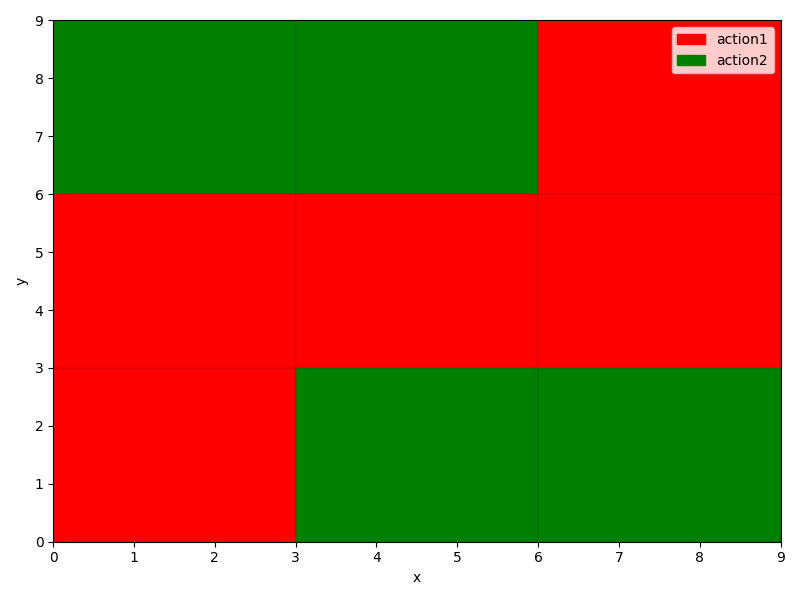
\includegraphics[width=\textwidth]{small_example}
        \subcaption{%
            % Tree representation of strategy with 2 state dimensions and 3
            % actions
        }\label{fig:smallExParts}
    \end{subfigure}
    \begin{subfigure}[b]{.5\textwidth}
        \centering
        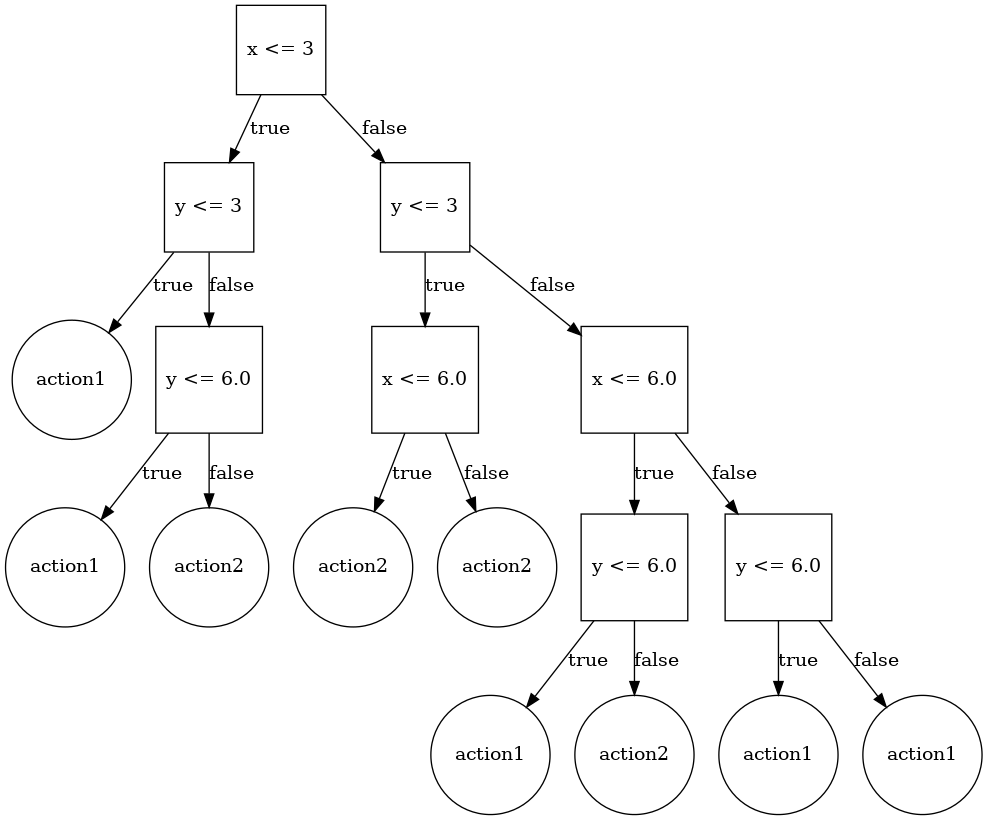
\includegraphics[width=\textwidth]{small_example_tree}
        \subcaption{%
            % 2D visualization of the state space partitioning entailed by the
            % decision tree.
        }\label{fig:smallExTree}
    \end{subfigure}%

    \caption{%
        An example of a state space partitioning \subref{fig:smallExParts}
        and a decision tree that induces it \subref{fig:smallExTree}.
    }%
    \label{fig:smallEx}
\end{figure}

\paragraph{The algorithm} The \textsc{MaxPartitions} algorithm generates a new
partitioning $\mathcal{A}'$ from $\mathcal{T}$ and its induced partitioning
$\mathcal{A}_{\mathcal{T}}$ whose regions (or \textit{partitions}) are as large
as possible while still respecting the singular mapping requirement in
$\mathcal{T}$. This is done by taking a region in the original partitioning and
expanding it in one dimension to the value of the closest next bound in that
dimension. We then evaluate this expanded region in $\mathcal{T}$ to see, if it
still has singular mapping. If it does not, we mark the dimension as exhausted,
revert the expansion and continue searching in unexhausted dimensions. If the
singular mapping requirement was not violated, we note that we have found a
larger, legal region and repeat the process until all dimensions have been
exhausted.

The algorithm operates through two loops: an inner loop, that tries to expand a
region until all dimensions have been exhausted, and an outer loop, that repeats
until the state space has been covered by new regions. In order to ensure a
feasible runtime, we need to bound the outer loop by the number of regions in
the original partitioning. This requires the algorithm to treat the case when an
expansion cuts a region from the original partitioning in more than
two.\footnote{%
    This cannot happen when the original partitioning is a grid (like in the
    example of Figure~\ref{fig:smallEx}), but will likely happen if the original
    regions are of different shapes and sizes.
} When this happens, the algorithm goes into a \textit{healing} mode, where it
has to remember the last legal region while it attempts to expand so far that it
subsumes the broken region(s). If this is not possible without violating the
singular mapping requirement, the healing has failed and the algorithm must
revert back to the last legal region and mark the dimension (in which the
breaking expansion happened) as exhausted.

Finally, we keep track of what areas of the state space have been covered by new
regions using a separate decision tree. Whenever the outer loop starts a new
iteration, we ask this \textit{tracking} tree for an uncovered region until the
entire state space is covered. The algorithm then returns a mapped partitioning,
that is guaranteed to have no more regions than the original partitioning.

\paragraph{Experiments} We conduct experiments on two types of cases: in the
first case, the input partitioning has a grid-like or tabular structure (like in
Figure~\ref{fig:smallEx}). The data will come from synthesized shields for
control of hybrid systems~\cite{brorholtShieldedReinforcementLearning2023}. In
the second case, the input partitionings will have an irregular structure, with
regions being of different shapes and sizes.\footnote{%
    All regions will however be rectangular.
} We use \textsc{UPPAAL Stratego}~\cite{davidUppaalStratego2015} to generate
near-optimal control strategies and then convert these to decision trees which,
because of the nature of how \textsc{UPPAAL} does its
partitioning~\cite{jaegerTeachingStrategoPlay2019}, exhibits highly irregular
regions and retains redundant information.

Table~\ref{tab:results} shows the results of repeatedly applying the
\textsc{MaxPartitions} algorithm on models of different types and
dimensionality. We apply the algorithm repeatedly until a fixpoint is reached.
\textsc{MaxPartitions} doesn't necessarily find a minimal partitioning, but it
does guarantee to not not increase the size of the input partitioning. 

Clearly, the algorithm can achieve substantial reductions in the
partitioning size, especially in the cases where the input partitionings have
been large. Since \textsc{MaxPartitions} retains the exact same state/action
mapping as the original mapped partitioning, there is a natural limit to how
few regions are needed.

\begin{table}[b]
    \centering
    \caption{%
        Results of repeatedly applying \textsc{MaxPartitions} on various types
        of input and models.
    }\label{tab:results}
    \begin{tabular}[t]{llcccc}
        \toprule
        Type & Model & State dimensions & Original size & New size & Iterations \\
        \midrule
        \multirow{2}*{Shield} & Bouncing ball & 2 & 700,000 & 1,352 & 3 \\
                              & Random walk & 2 & 57,600 & 35 & 1 \\
        \midrule
        \multirow{5}*{Strategy} & Bouncing ball & 2 & 81,747 & 696 & 4 \\
                                & Cartpole & 4 & 76,993 & 3,898 & 10 \\
                                & Cruise & 2 & 436 & 173 & 2 \\
                                & Traffic light & 5 & 436 & 110 & 5 \\
                                & DCDC boost controller & 3 & 5,652 & 433 & 4 \\
        \bottomrule
    \end{tabular}
\end{table}

\newpage

\bibliographystyle{ieeetr}
\bibliography{references}

\end{document}

% \[
%     \text{MaxPart}(\mathcal{T}_1, \mathcal{A}_{\mathcal{T}_1}) \rightarrow
%     \mathcal{A}' \rightarrow
%     \text{Tree}(\mathcal{A}') \rightarrow
%     \mathcal{T}_2 \rightarrow
%     \text{MaxPart}(\mathcal{T}_{2}, \mathcal{A}_{\mathcal{T}_2}) \rightarrow
%     \mathcal{A}'' \rightarrow
%     \text{Tree}(\mathcal{A}'') \rightarrow
%     \mathcal{T}_3 \rightarrow
%     \ldots
% \] 

